%IMD PNA http://na.support.keysight.com/pna/help/latest/Applications/Swept_IMD_Configure_External_Source_and_Combiner.htm
\chapter{Desarrollo}

%%-----------------------------------------------------------------------

\section{Desarrollo del proyecto}

\subsection{Datos}

La base de datos de archivos MIDI que se utilizo en este proyecto se llama ''Clean MIDI subset'' la cual se uso en la tesis doctoral \cite{Lear_Coli}. Esta base de datos contiene m�s de 17,000 canciones en formato MIDI, estas en su mayor�a del g�nero Pop y Rock, por lo que la red utilizada en este proyecto fue entrenada para asimilar este tipo de estilos.

Para el procesamiento de los archivos MIDI se utilizo una librer�a de software libre llamada Music21, la cual nos permite de una manera f�cil trabajar con estos archivos, sin embargo se realizo una adaptacion para que funcionara correctamente con diferentes sonidos de guitarra y bajo el�ctrico. Esta librer�a es compatible con Python3 por lo que nuestro programa esta hecho en este lenguaje de programaci�n.

Los archivos MIDI de esta base de datos poseen varios Tracks, cada uno con un instrumento diferente, de los cuales en este proyecto solamente se tomaran en cuenta los Tracks de guitarra y bajo el�ctrico, los demas Tracks ser�n ignorados.

Cada canci�n tiene una duraci�n promedio de 3 minutos, por lo que la cantidad de notas que procesa la red es bastante considerable.

\subsection{Arquitectura de la aplicaci�n}

Este proyecto posee varios modulos, cada uno funciona independientemente de los otros, sin embargo existen interconexiones entre ellos para el paso de informaci�n, esto nos permite tener una buena modulaci�n del c�digo y realizar cambios en un modulo sin afectar a los otros.

Estos modulos se pueden observar en la siguiente figura:

\begin{figure}[H]
	\centerline{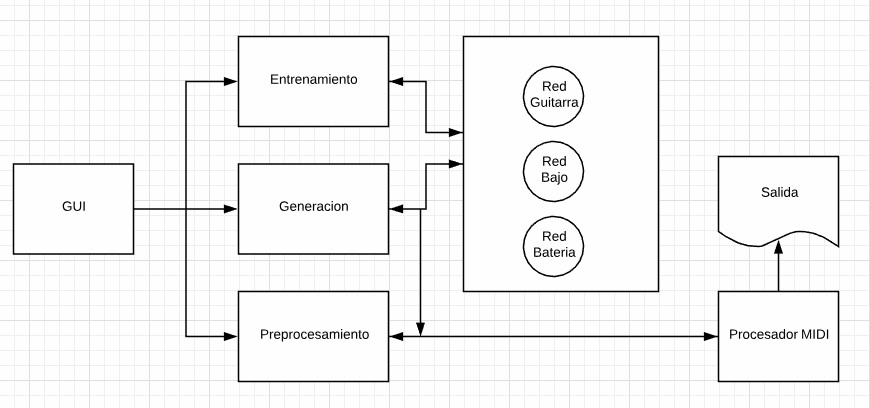
\includegraphics[width=14cm]{arq_app.png}}
	\caption{Arquitectura de la aplicaci�n}
	\label{fig:arq_app}
\end{figure}

Dentro de esta arquitectura tenemos modulos activos y modulos pasivos. Los modulos activos son aquellos que reciben y procesan informaci�n, mientras que los elementos pasivos solamente son para almacenar o consultar informaci�n. 

Los elementos activos que se observan son:

\begin{itemize}
	\item UI.
	\item Preprocesamiento.
	\item Red neuronal. 
	\item Entrenamiento.
	\item Generaci�n.  
	\item Analizador.
\end{itemize}

Mientras que los elementos pasivos son:

\begin{itemize}
	\item Base de datos.
	\item Datos preprocesados.
	\item Canciones generadas.
\end{itemize}

A continuaci�n se describir�n cada modulo del sistema.

\subsubsection{UI}

Este modulo es una peque�a interfaz de usuario de consola basada en menus, la cual nos permite accesar a los otros modulos del sistema.

El menu principal contiene el acceso a los siguientes modulos:

\begin{enumerate}
	\item Preprocesamiento.
	\item Entrenamiento.
	\item Generaci�n.  
	\item Analizador.
\end{enumerate}

Como se puede observar en la figura \ref{fig:arq_app} hay algunos modulos que para poderse ejecutar es necesario ejecutar otro modulo primero, con el fin de obtener la informaci�n necesaria para este modulo. El �nico modulo que no tiene condicionantes es el de Preprocesamiento, por lo tanto es el primer modulo que se deber�a de ejecutar en el programa.

\subsubsection{Preprocesamiento}

\subsubsection{Red neuronal}

\subsubsection{Entrenamiento}

\subsubsection{Generaci�n}

\subsubsection{Analizador}

\section{Resultados}